% CODIGO DE ORDENACIONES
\definecolor{lightergray}{RGB}{247,247,247}
\definecolor{darkgreen}{RGB}{36,135,20}
\definecolor{green_comment}{RGB}{0,128,0}
\definecolor{redcell}{RGB}{238,176,176}
\definecolor{greencell}{RGB}{217,234,211}

\newpage
% GRAFICA DE HISOGRAMA COLOR ENCIMA DE OTRO
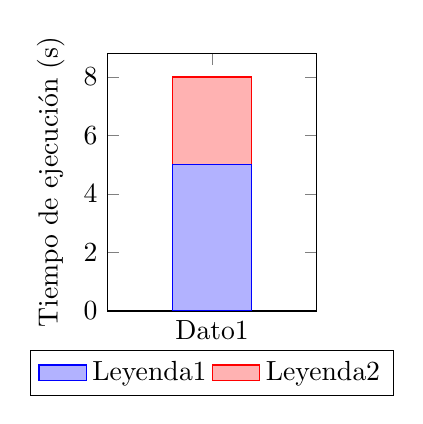
\begin{tikzpicture}
	\begin{axis}[
		ybar stacked,
		bar width=1cm, % Increased bar width
		ylabel={Tiempo de ejecución (s)},
		xlabel={Datos},
		symbolic x coords={Dato1},
		xtick=data,
		enlarge x limits=0.15,
		ymin=0,
		width=0.35\textwidth, % Reduced width
		height=0.4\textwidth, % Reduced height
		legend style={at={(0.5,-0.15)}, anchor=north, legend columns=-1},
		area legend
		]
		
		\addplot+[ybar] plot coordinates {(Dato1, 5) };
		\addplot+[ybar] plot coordinates {(Dato1, 3) };
		
		
		
		\legend{Leyenda1, Leyenda2}
		
		
	\end{axis}
\end{tikzpicture}

% DOS GRAFICAS EN UNA
\begin{figure}[h!]
	\centering
	\begin{tikzpicture}
		% Define custom colors
		\definecolor{myblue}{RGB}{0, 114, 178}
		\definecolor{myorange}{RGB}{213, 94, 0}
		
		% Memory Usage plot
		\begin{axis}[
			name=grafico_memoria,
			title={Memoria con el paso del tiempo},
			xlabel={Tiempo (s)},
			ylabel={Uso de Memoria (MB)},
			grid=major,
			width=0.35\textwidth, % Reduced width
			height=0.4\textwidth, % Reduced height
			xmin=0, xmax=60,
			ymin=0, ymax=1024,
			xtick={0,10,...,60},
			ytick={0,200,...,1024},
			yticklabel style={/pgf/number format/fixed},
			legend pos=north west,
			grid style=dashed,
			]
			% Blue line
			\addplot[
			name path=blue,
			color=myblue,
			mark=square,
			]
			coordinates {
				(0, 200)
				(10, 300)
				(20, 400)
				(30, 500)
				(40, 700)
				(50, 900)
				(60, 1000)
			};
			\addlegendentry{Memoria - Azul}
			
			% Orange line
			\addplot[
			name path=orange,
			color=myorange,
			mark=triangle,
			]
			coordinates {
				(0, 100)
				(10, 200)
				(20, 300)
				(30, 400)
				(40, 600)
				(50, 800)
				(60, 900)
			};
			\addlegendentry{Memoria - Naranja}
			
			% Fill area between blue and orange lines
			\addplot [
			color=myblue!50, 
			fill=myblue!50, 
			fill opacity=0.3
			]            
			fill between [
			of=blue and orange,
			soft clip={domain=0:60},
			];
			
			% Fill area between orange line and x-axis
			\addplot [
			name path=axis,
			draw=none,
			]
			coordinates {
				(0,0)
				(10,0)
				(20,0)
				(30,0)
				(40,0)
				(50,0)
				(60,0)
			};
			
			\addplot [
			color=myorange!50, 
			fill=myorange!50, 
			fill opacity=0.3
			]            
			fill between [
			of=orange and axis,
			soft clip={domain=0:60},
			];
		\end{axis}
		
		% Execution Time plot
		\begin{axis}[
			name=ejecucion,
			at={(grafico_memoria.east)},
			anchor=west,
			title={Tiempo usado},
			ybar stacked,
			bar width=0.7cm, % Reduced bar width
			ylabel={Tiempo de Ejecución (s)},
			xlabel={Datos},
			symbolic x coords={Dato1},
			xtick=data,
			enlarge x limits=0.15,
			ymin=0,
			width=0.35\textwidth, % Reduced width
			height=0.4\textwidth, % Reduced height
			legend style={at={(0.5,-0.15)}, anchor=north, legend columns=-1},
			area legend
			]
			
			\addplot+[ybar, myblue, fill=myblue!50] plot coordinates {(Dato1, 5) };
			\addplot+[ybar, myorange, fill=myorange!50] plot coordinates {(Dato1, 3) };
			
			\legend{Phase 1, Phase 2}
		\end{axis}
	\end{tikzpicture}
	\caption{Comparacion de la memoria y tiempo de ejecución.}
	\label{fig:comparison}
\end{figure}
% DOS GRAFICAS EN UNA (MEJORADO)
\begin{figure}
	\centering
	\begin{subfigure}[b]{0.45\textwidth}
		\centering
		\begin{tikzpicture}
			\begin{axis}[
				title={Memoria con el paso del tiempo},
				xlabel={Tiempo (s)},
				ylabel={Uso de Memoria (MB)},
				grid=major,
				width=\textwidth,
				height=0.6\textwidth, % Adjusted height
				xmin=0, xmax=60,
				ymin=0, ymax=1024,
				xtick={0,10,...,60},
				ytick={0,200,...,1024},
				yticklabel style={/pgf/number format/fixed},
				legend pos=north west,
				grid style=dashed,
				]
				% Blue line
				\addplot[
				name path=blue,
				color=blue,
				mark=square,
				]
				coordinates {
					(0, 200)
					(10, 300)
					(20, 400)
					(30, 500)
					(40, 700)
					(50, 900)
					(60, 1000)
				};
				\addlegendentry{Memoria - Blue)}
				
				% Orange line
				\addplot[
				name path=orange,
				color=orange,
				mark=triangle,
				]
				coordinates {
					(0, 100)
					(10, 200)
					(20, 300)
					(30, 400)
					(40, 600)
					(50, 800)
					(60, 900)
				};
				\addlegendentry{Memoria Naranja}
				
				% Fill area between blue and orange lines
				\addplot [
				color=blue!50, 
				fill=blue!50, 
				fill opacity=0.3
				]            
				fill between [
				of=blue and orange,
				soft clip={domain=0:60},
				];
				
				% Fill area between orange line and x-axis
				\addplot [
				name path=axis,
				draw=none,
				]
				coordinates {
					(0,0)
					(10,0)
					(20,0)
					(30,0)
					(40,0)
					(50,0)
					(60,0)
				};
				
				\addplot [
				color=orange!50, 
				fill=orange!50, 
				fill opacity=0.3
				]            
				fill between [
				of=orange and axis,
				soft clip={domain=0:60},
				];
				
			\end{axis}
		\end{tikzpicture}
		\caption{Memoria con el paso del tiempo.}
		\label{fig:memory_usage}
	\end{subfigure}
	\begin{subfigure}[b]{0.45\textwidth}
		\centering
		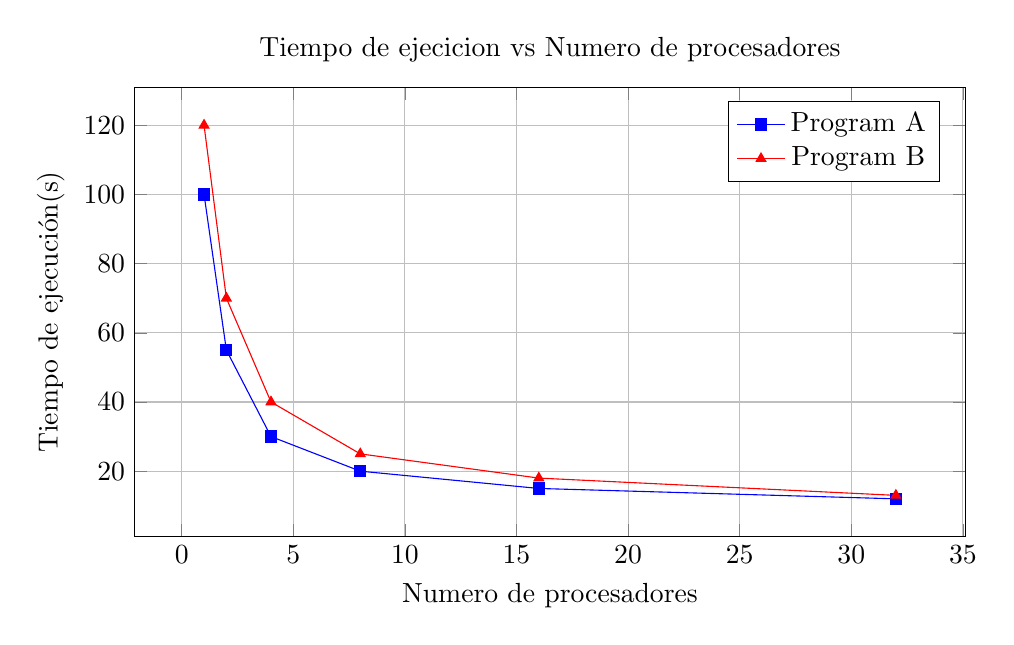
\begin{tikzpicture}
			\begin{axis}[
				title={Tiempo de ejecicion vs Numero de procesadores},
				xlabel={Numero de procesadores},
				ylabel={Tiempo de ejecución(s)},
				legend pos=north east,
				grid=major,
				width=\textwidth,
				height=0.6\textwidth % Adjusted height
				]
				% Sample data
				\addplot[color=blue, mark=square*] coordinates {
					(1, 100)
					(2, 55)
					(4, 30)
					(8, 20)
					(16, 15)
					(32, 12)
				};
				\addlegendentry{Program A}
				
				\addplot[color=red, mark=triangle*] coordinates {
					(1, 120)
					(2, 70)
					(4, 40)
					(8, 25)
					(16, 18)
					(32, 13)
				};
				\addlegendentry{Program B}
				
			\end{axis}
		\end{tikzpicture}
		\caption{Tiempo de ejecución para diferenntes numeros de procesadores}
		\label{fig:execution_time}
	\end{subfigure}
	
	
	\caption{Dos gráficos al lado}
	\label{fig:twoplots}
\end{figure}


\newpage

\begin{verbatim}
	n		 # int. Tam. de la poblacion
	d		 # int. Numero de variables/dimensiones
	K		 # int. Numero de Centroides
	poblacion	 # float[n]. Individuos 
	centroides	 # float[K]. Centroides
	asignacion	 # float[n]. Asignacion para cada individuo
	
	indsCluster	 # float[K]. Numero de individuos para cada centroide
	centroidesNuevos # float[K]. Centroides calculados en la iteracion
\end{verbatim}

\begin{algorithm}
	\caption{Euclid's algorithm}
	\KwData{Two nonnegative integers $a$ and $b$}
	\KwResult{$\gcd(a,b)$}
	\While{$b \neq 0$}{
		$r \leftarrow a \bmod b$\;
		$a \leftarrow b$\;
		$b \leftarrow r$\;
	}
	\Return $a$\;
\end{algorithm}

\newpage

\chapter{Estudio empírico}

Después de implementar y diseñar los algoritmos y mejoras utilizando MPI, llevamos a  cabo un análisis exhaustivo para evaluar los tiempos de ejecución, realizar pruebas, contrastar resultados y extraer conclusiones.

Primero se ejecutan distintas pruebas en un ordenador normal, para luego ejecutar las mejores implementaciones en un cluster con varios ordenadores y muchos procesos.



\begin{tcolorbox}[boxrule=0.5pt, fontupper=\small]
\scriptsize
\textcolor{red}{
Ordenador básico: 8 núcleos, 16 procesos lógicos y 32gb de ram\\
\\
\\
\\
Cluster:
\\
}
\end{tcolorbox}
	



% ------------------------------------------------------------------------------------------------
% --- ORDENACIONES  ------------------------------------------------------------------------------
% ------------------------------------------------------------------------------------------------


% VARIABLES Y PRUEBAS DE ORDENACIONES 
\begin{flushleft}
\textbf{Ordenaciones}
\begin{mdframed}[roundcorner=5pt]
\textbf{\underline{Pruebas}}
\vspace{0.1cm}

\scriptsize	
\textbf{Arrays de enteros, siempre en el caso peor,} es decir, ordenados de forma \textbf{decreciente}, por lo que tiene que ejecutar el mayor número de comparaciones para ordenarlo de forma creciente.\\	
Las pruebas se ejecutan sobre el mismo array de enteros, y se van aumentando el tamaño para medir los tiempos de ejecución. En cada prueba se añaden \textit{x} elementos más a ordenar.
\begin{tcolorbox}[boxrule=0.5pt, fontupper=\small]
	\scriptsize
	El incremento del tamaño viene dado de la siguiente forma:\\
	- [20-1.000) $\rightarrow$ 20 elementos.\\
	- [1.000-10.000) $\rightarrow$ 250 elementos.\\
	- [10.000-100.000) $\rightarrow$ 1.000 elementos.\\
	Para MergeSort, al ser un algoritmo mas eficiente, no se añade de mil en mil al llegar a 10.000 elementos, se mantiene el incremento de 250 elementos.

\end{tcolorbox}

\end{mdframed}
\end{flushleft}

\newpage

\begin{figure}[h]
	\centering
	\begin{tikzpicture}
		\begin{axis}[
			xlabel={Tam. Array ($10^4$)},
			ylabel={Tiempo (s)},
			legend pos=north west,
			grid=major,
			width=\textwidth,
			height=0.6\textwidth
			]
			
			% Plot data from the file without markers, with different colors, and thicker lines
			\addplot [mark=none, color=red, line width=1.2pt] table [x index=0, y index=1, col sep=space] {files/sortn2.txt};
			\addplot [mark=none, color=blue, line width=1.2pt] table [x index=0, y index=2, col sep=space] {files/sortn2.txt};
			\addplot [mark=none, color=darkgreen, line width=1.2pt] table [x index=0, y index=3, col sep=space] {files/sortn2.txt};
			\addplot [mark=none, color=green, line width=1.2pt] table [x index=0, y index=4, col sep=space] {files/sortn2.txt};
			\addplot [mark=none, color=black, line width=1.2pt] table [x index=0, y index=5, col sep=space] {files/sortn2.txt};
			
			% Add legends
			\addlegendentry{BubbleSort}
			\addlegendentry{InsertionSort}
			\addlegendentry{SelectionSort}
			\addlegendentry{SequentialSort }
			\addlegendentry{SequentialSort\_MPI(5)}
			
		\end{axis}
	\end{tikzpicture}
	\caption{Tiempo de ejecución de los algoritmos de ordenación cuadráticos}
\end{figure}

La implementación aplicando MPI sobre SequentialSort tiene un speed-up proporcional al número de procesos ejecutándose al llegar a un cierto número de elementos a ordenar.  %TODO
Al paralelizar el trabajo de SequentialSort, se pueden obtener mejores resultados que SelectionSort al usar cinco o más procesos workers.

De las ordenaciones básicas con coste cuadrático (O(N2)) comentadas anteriormente, SelectionSort es la que mejores resultados obtiene, y BubbleSort la peor, siendo aproximadamente 3.5 veces más lenta con 70.000 elementos. 
La ordenación diseñada SequentialSort es incluso más rápida que dos de las más famosas, debido a la simpleza de las operaciones aplicadas en la ordenación. Esta ordenación hace N2 comparaciones, pero al no modificar elementos del array sigue siendo más rápida que las otras.


\lstset{language=python, 
	breaklines=true, 
	basicstyle=\footnotesize,
	backgroundcolor=\color{lightergray}}	
\begin{lstlisting}[frame=single]
	def selection_sort(a):			def sequential_sort(a):
	n = len(a)				  INF=sys.maxsize
	minE = 0				  n=len(a)
	pos = 0			  	  b=[(INF) for i in range(n)]  
	
	for i in range(n-1):			  for i in range(n):
	minE = a[i]			    cont=0
	pos = i				    val=a[i]
	for j in range(i+1, n):		    for i in range(n):  
	if minE > a[j]:		      if a[i]<val: cont+=1
	minE = a[j]				while b[cont]!=INF: 
	pos = j				  cont+=1
	b[cont]=val
	tmp = a[i]
	a[i] = a[pos]
	a[pos] = tmp
	
\end{lstlisting}
\newpage

%Sequential sort + Uso de memoria
\begin{figure}[h!]
	\centering
	\begin{tikzpicture}
		\begin{groupplot}[group style={
				group size=2 by 1,
				horizontal sep=1.5cm, % Adjust horizontal separation between plots
				vertical sep=0.5cm}, % Adjust vertical separation between plots           
			grid=major,
			width=0.45\textwidth, height=0.45\textwidth, % Adjust size as needed      
			tick label style={font=\tiny} % Adjust font size of tick labels  
			]
			
			% First plot
			\nextgroupplot[
			title={}, 
			ylabel=Tiempo \tiny de ejecución (s), 
			xlabel=Tam. Array,
			legend pos=north west
			]
			\addplot [mark=none, color=red, line width=1.2pt] table [x index=0, y index=1, col sep=space] {files/sequential.txt};
			\addplot [mark=none, color=black, line width=1.2pt] table [x index=0, y index=2, col sep=space] {files/sequential.txt};
			\addplot [mark=none, color=darkgreen, line width=1.2pt] table [x index=0, y index=3, col sep=space] {files/sequential.txt};
			
			% Add legends
			\addlegendentry{Básico}
			\addlegendentry{MPI\_1}
			\addlegendentry{MPI\_2}
			
			% Second plot
			\nextgroupplot[
			title={},
			xtick={2,3,4,5,6,7,8,9,10}, % Adjust x-tick positions as needed
			ytick={0,2,4,6,8,10,12}, % Adjust y-tick positions as needed
			legend pos=north west,			
			xlabel=Num. Procesadores,
			ylabel=Memoria \tiny(Copias del array)
			]
			\addplot[name path=blue, color=blue, mark=square] table {files/sequentialMem.txt};
			\addlegendentry{MPI\_1}
			
			\addplot[name path=orange, color=orange, mark=triangle] table [y index=2] {files/sequentialMem.txt};
			\addlegendentry{MPI\_2}
			
			\addplot [color=blue!50, fill=blue!50, fill opacity=0.3] fill between [of=blue and orange, soft clip={domain=2:10}];
			
			\addplot [name path=axis, draw=none] coordinates {(2,0) (10,0) };	
			
			\addplot [color=orange!50, fill=orange!50, fill opacity=0.3] fill between [of=orange and axis, soft clip={domain=2:10}];
			
		\end{groupplot}  
		
	\end{tikzpicture}
	\caption{Mejoras MPI SequentialSort + Memoria}
\end{figure}


% HISTOGRAMA CON VARIOS PROCESOS
\begin{figure}[h!]
\begin{tikzpicture}
	\begin{axis}[
		ybar,
		bar width=0.35cm,
		ylabel={Tiempo de ejecución (s)},
		xlabel={Tamaño del array (miles de elementos)},
		symbolic x coords={25, 50, 75, 100},
		xtick=data,
		enlarge x limits=0.2,
		ymin=0,
		%width=15cm,
		%height=10cm,
		width=\textwidth,
		height=0.45\textwidth,
		legend style={at={(0.5,-0.15)}, anchor=north, legend columns=-1},
		area legend
		]
		
		\addplot+[ybar, pattern=vertical lines, draw=black] plot coordinates 
		{(25, 1.12) (50, 4.39) (75, 10.0) (100, 21)};
		\addplot+[ybar, pattern=grid, draw=black] plot coordinates 
		{(25, 0.67) (50, 2.58) (75, 5.70) (100, 10.15) };
		\addplot+[ybar, pattern=dots, draw=black] plot coordinates 
		{(25, 0.23) (50, 0.93) (75, 2.09) (100, 3.35) };
		\addplot+[ybar, pattern=crosshatch, draw=black] plot coordinates 
		{(25, 0.09) (50, 0.34) (75, 0.72) (100, 1.39)};
		\addplot+[ybar, pattern=checkerboard, draw=black] plot coordinates 
		{(25, 0.059) (50, 0.18) (75, 0.41) (100, 0.71)};
		
		
		\legend{Secuencial, MPI(4),MPI(8),MPI(16),MPI(32)}
	\end{axis}	
\end{tikzpicture}
\caption{Tiempo de ejecución MergeSort + MPI}
\end{figure}


\newpage

% ------------------------------------------------------------------------------------------------
% --- MATRIZ -------------------------------------------------------------------------------------
% ------------------------------------------------------------------------------------------------



% ------------------------------------------------------------------------------------------------
% --- JERARQUICO AGLOMERATIVO --------------------------------------------------------------------
% ------------------------------------------------------------------------------------------------
\newpage

\begin{flushleft}
\textbf{Algoritmos de Agrupación}
	\begin{mdframed}[roundcorner=5pt]
		\textbf{\underline{Pruebas}}
		\vspace{0.1cm}
		
		\scriptsize	
		\textbf{Las poblaciones que se usan en cada algoritmo se han generado previamente de manera aleatoria}, delimitando un intervalo [-10, 10] para todas las dimensiones disponibles. Para crear los gráficos se ejecutó muchas veces con diferentes tamaños para guardar los tiempos de ejecución con poblaciones de diferentes tamaños. Se añaden \textit{x} elementos a las poblaciones.
		
		
		\begin{tcolorbox}[boxrule=0.5pt, fontupper=\small]
			\scriptsize
			Para las implementaciones de K-Medias y Jerárquico Aglomerativo se aplican el mismo incremento que en las ordenaciones:
			El incremento del tamaño viene dado de la siguiente forma:\\
			- [20-1.000) $\rightarrow$ 20 elementos.\\
			- [1.000-10.000) $\rightarrow$ 250 elementos.\\
			- [10.000-100.000) $\rightarrow$ 1.000 elementos.\\
			
			Para K-Vecinos más cercanos (KNN), al ser un algoritmo lineal, se guarda el tiempo de ejecución cada veinte nuevos individuos categorizados.
			
		\end{tcolorbox}
		
	\end{mdframed}
\end{flushleft}





% JERARQUICO AGLOMERATIVO (EUCLIDEA y MANHATTAN)
\begin{figure}[!h]
	\centering
	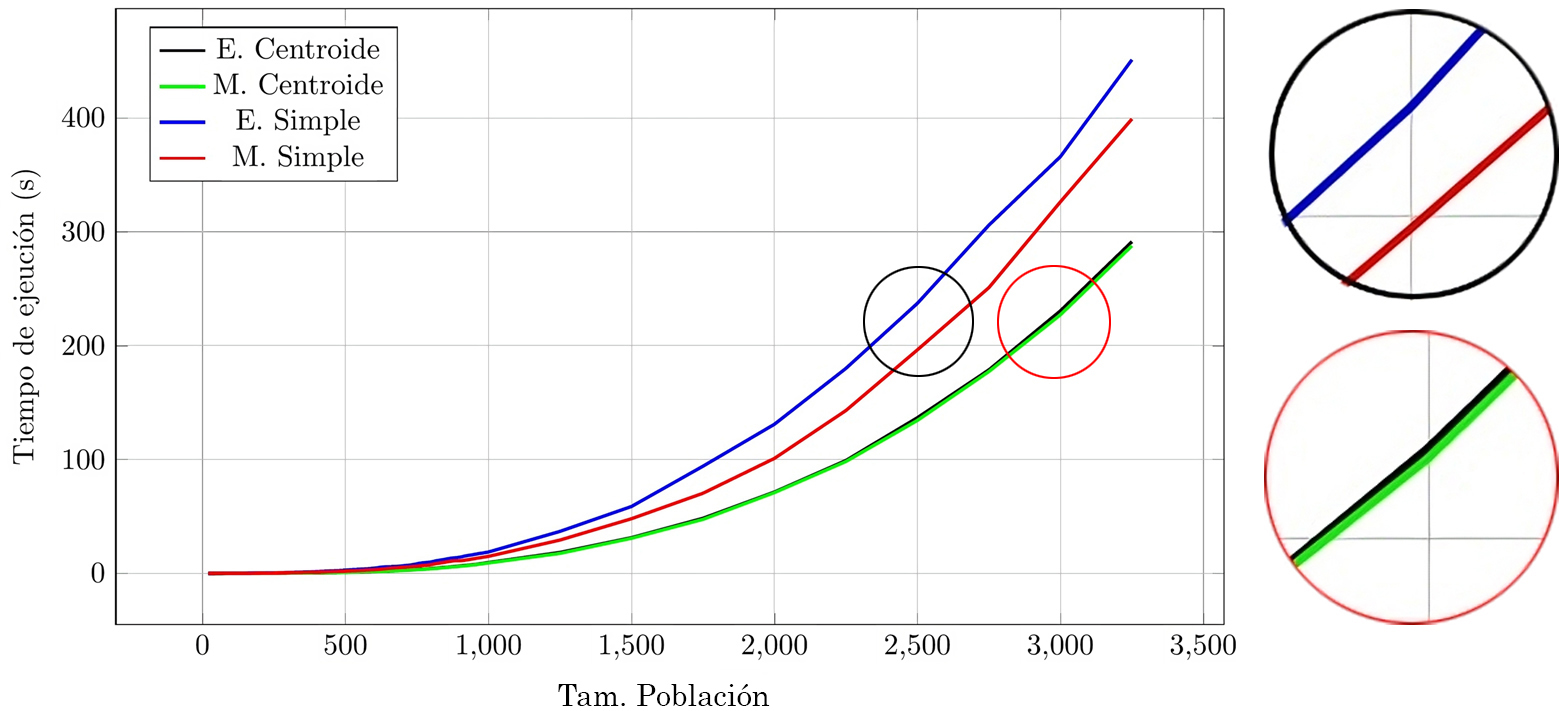
\includegraphics[width=0.8\textwidth]{images/jerarquico}
	\caption{Tiempo de ejecución del algoritmo básico Jerarquíco Aglomerativo}
	\label{fig:example}
\end{figure}



% JERARQUICO AGLOMERATIVO: HISTOGRAMA CON VARIOS PROCESOS
\begin{tikzpicture}
	\begin{axis}[
		ybar,
		bar width=0.35cm,
		ylabel={Tiempo de ejecución (s)},
		xlabel={Tam. Array},
		symbolic x coords={1000, 2500, 5000},
		xtick=data,
		enlarge x limits=0.2,
		ymin=0,
		width=15cm,
		height=10cm,
		legend style={at={(0.5,-0.15)}, anchor=north, legend columns=-1},
		area legend
		]
		
		\addplot+[ybar, pattern=vertical lines, draw=black] plot coordinates 
		{(1000, 7.61) (2500, 141.59) (5000, 1098.29)};
		\addplot+[ybar, pattern=grid, draw=black] plot coordinates 
		{(1000, 4.81) (2500, 79.61) (5000, 617.44)};
		\addplot+[ybar, pattern=dots, draw=black] plot coordinates 
		{(1000, 2.75) (2500, 47.36) (5000, 379.42) };
		\addplot+[ybar, pattern=crosshatch, draw=black] plot coordinates 
		{(1000, 2.24) (2500, 38.55) (5000, 304.12) };
		\addplot+[ybar, pattern=checkerboard, draw=black] plot coordinates 
		{(1000, 1.98) (2500, 33.13) (5000, 260.77)};
		
		
		\legend{Secuencial, MPI(2),MPI(4),MPI(6),MPI(8)}
	\end{axis}
\end{tikzpicture}

\newpage
% ------------------------------------------------------------------------------------------------
% --- KMEDIAS ------------------------------------------------------------------------------------
% ------------------------------------------------------------------------------------------------
\textbf{K-MEDIAS}
\begin{figure}[!h]
	\centering
	\begin{tikzpicture}
		\begin{axis}[
			xlabel={Tam. Población ($10^5$)},
			ylabel={Tiempo de ejeución (s)},
			legend pos=north west,
			grid=major,
			width=\textwidth,
			height=0.6\textwidth
			]
			
			% Plot data from the file without markers, with different colors, and thicker lines
			\addplot [mark=none, color=blue, line width=1.2pt] table [x index=0, y index=1, col sep=space] {files/kmedias.txt};
			\addplot [mark=none, color=red, line width=1.2pt] table [x index=0, y index=2, col sep=space] {files/kmedias.txt};
			\addplot [mark=none, color=darkgreen, line width=1.2pt] table [x index=0, y index=3, col sep=space] {files/kmedias.txt};
			\addplot [mark=none, color=black, line width=1.2pt] table [x index=0, y index=4, col sep=space] {files/kmedias.txt};
			
			
			% Add legends
			\addlegendentry{Euclidea}
			\addlegendentry{Manhattan}
			\addlegendentry{Euclidea\_MPI}
			\addlegendentry{Manhattan\_MPI}
			
			
		\end{axis}
	\end{tikzpicture}
	\caption{Tiempo de ejecución para KMedias}
\end{figure}





\begin{figure}
	\centering
	\begin{tikzpicture}
		\begin{axis}[
			xlabel={Tam. Población},
			ylabel={SpeedUp},
			legend pos=north east,
			grid=major,
			width=0.85\textwidth,
			height=0.45\textwidth
			]
			
			% Plot data from the file without markers, with different colors, and thicker lines
			\addplot [mark=none, color=darkgreen, line width=1.7pt] table [x index=0, y index=1, col sep=space] {files/kmedias_speedup.txt};
			\addplot [mark=none, color=red, line width=0.3pt] table [x index=0, y index=2, col sep=space] {files/kmedias_speedup.txt};
			\addplot [mark=none, color=blue, line width=0.3pt] table [x index=0, y index=3, col sep=space] {files/kmedias_speedup.txt};
			
			
			% Add legends
			\addlegendentry{Ideal}
			\addlegendentry{Euclidea}
			\addlegendentry{Manhttan}
			
			
		\end{axis}
	\end{tikzpicture}
	\caption{SpeedUp - KMedias}
\end{figure}

\newpage


% KMEDIAS: HISTOGRAMA CON VARIOS PROCESOS
\begin{figure}[!h]
	\centering
	\begin{tikzpicture}
		\begin{axis}[
			width=\textwidth,
			height=10cm,
			ybar,
			bar width=0.35cm,
			ylabel={Tiempo de ejecución (s)},
			xlabel={Tam. de la Población},
			symbolic x coords={25000, 50000, 75000, 100000},
			xtick=data,
			enlarge x limits=0.2,
			ymin=0,
			legend style={at={(0.5,-0.15)}, anchor=north, legend columns=-1},
			area legend,
			legend columns=4,
			]
			
			% Histo
			\addplot+[ybar, pattern=vertical lines, draw=black] plot coordinates 
			{(25000, 0.62) (50000, 1.31) (75000, 1.66) (100000, 2.56)};				
			\addplot+[ybar, pattern=grid, draw=black] plot coordinates 
			{(25000, 1.69) (50000, 4.22) (75000, 5.19)  (100000, 8.76)};						
			\addplot+[ybar, pattern=dots, draw=black] plot coordinates 
			{(25000, 8.29) (50000, 33.80) (75000, 79.83) (100000, 79.56)};						
			\addplot+[ybar, pattern=crosshatch, draw=black] plot coordinates 
			{(25000, 19.93) (50000, 56.03) (75000, 109.96) (100000, 123.16)};
			
			\addplot[smooth, mark=diamond, green] plot coordinates
			{(25000, 0.62) (50000, 1.31) (75000, 1.66) (100000, 2.56)};
			\addplot[smooth, mark=diamond, blue] plot coordinates
			{(25000, 1.69) (50000, 4.22) (75000, 5.19)  (100000, 8.76)};
			\addplot[smooth, mark=diamond, black] plot coordinates
			{(25000, 8.29) (50000, 33.80) (75000, 79.83) (100000, 79.56)};
			\addplot[smooth, mark=diamond, red] plot coordinates
			{(25000, 19.93) (50000, 56.03) (75000, 109.96) (100000, 123.16)};
			
			\legend{5, 10, 25, 50}
		\end{axis}
	\end{tikzpicture}
	\caption{KMedias variando K}
\end{figure}



\newpage
% ------------------------------------------------------------------------------------------------
% --- KNN ----------------------------------------------------------------------------------------
% ------------------------------------------------------------------------------------------------

\textbf{KNN}

% KNN BASICO
\begin{figure}[h!]
	\centering
	\begin{tikzpicture}
		\begin{axis}[
			xlabel={Tam. Población ($10^5$)},
			ylabel={Tiempo de ejeución (s)},
			legend pos=north west,
			legend columns=2,
			grid=major,
			width=\textwidth,
			height=0.6\textwidth
			]
			
			% Plot data from the file without markers, with different colors, and thicker lines
			\addplot [mark=none, color=darkgreen, line width=1.2pt] table [x index=0, y index=1, col sep=space] {files/knn.txt};
			\addplot [mark=none, color=red, line width=1.2pt] table [x index=0, y index=3, col sep=space] {files/knn.txt};
			\addplot [mark=none, color=black, line width=1.2pt] table [x index=0, y index=2, col sep=space] {files/knn.txt};
			
			\addplot [mark=none, color=blue, line width=1.2pt] table [x index=0, y index=4, col sep=space] {files/knn.txt};
			
			
			% Add legends
			\addlegendentry{Euclidea}
			\addlegendentry{Euclidea\_Act}
			\addlegendentry{Manhattan}
			
			\addlegendentry{Manhattan\_Act}
			
			
		\end{axis}
	\end{tikzpicture}
	\caption{Tiempo de ejecución para KNN}
\end{figure}


\begin{figure}[!h]
	\centering
	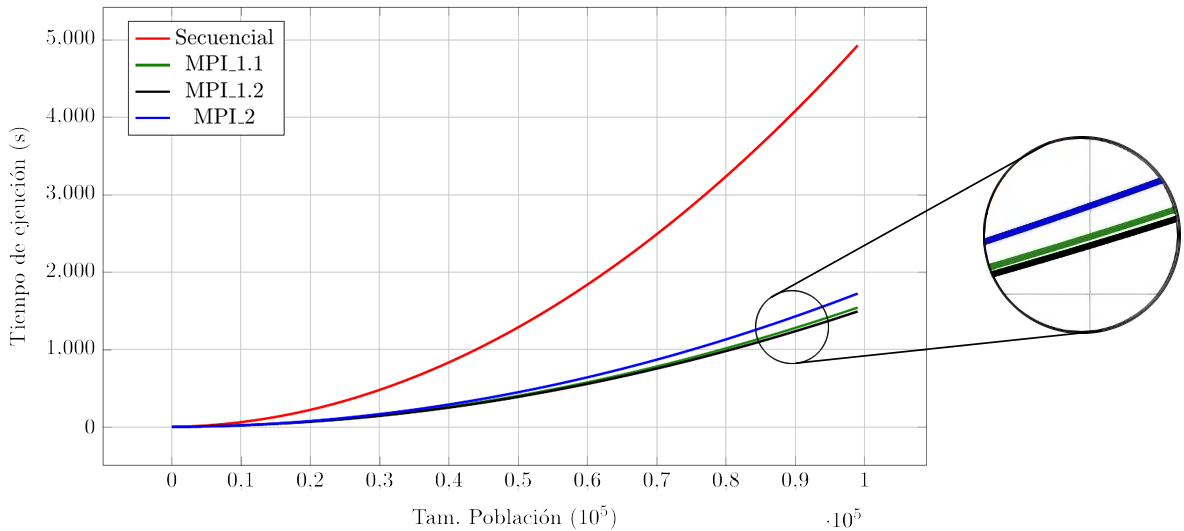
\includegraphics[width=0.8\textwidth]{images/knn_mpi}
	\caption{Tiempo de ejecución del algoritmo básico Jerarquíco Aglomerativo}
	\label{fig:example}
\end{figure}


\newpage


\begin{figure}
	\centering
	\begin{tikzpicture}
		\begin{axis}[
			xlabel={Tam. Población},
			ylabel={SpeedUp},
			legend pos=south east,			
			legend columns=3,
			grid=major,
			width=0.85\textwidth,
			height=0.45\textwidth
			]
			
			% Plot data from the file without markers, with different colors, and thicker lines
			\addplot [mark=none, color=darkgreen, line width=0.8pt] table [x index=0, y index=1, col sep=space] {files/knn_speedup.txt};
			\addplot [mark=none, color=red, line width=0.8pt] table [x index=0, y index=2, col sep=space] {files/knn_speedup.txt};
			\addplot [mark=none, color=blue, line width=0.8pt] table [x index=0, y index=3, col sep=space] {files/knn_speedup.txt};
			
			
			% Add legends
			\addlegendentry{Ideal}
			\addlegendentry{MPI\_1}
			\addlegendentry{MPI\_2}
			
			
		\end{axis}
	\end{tikzpicture}
	\caption{SpeedUp - KNN}
\end{figure}

\newpage
% KNN MPI
%\begin{figure}
%\centering
%\begin{tikzpicture}
%	\begin{axis}[
%		xlabel={Tam. Población ($10^5$)},
%		ylabel={Tiempo de ejeución (s)},
%		legend pos=north west,
%		grid=major,
%		width=\textwidth,
%		height=0.6\textwidth
%		]
%		
%		% Plot data from the file without markers, with different colors, and thicker lines
%		\addplot [mark=none, color=red, line width=1.2pt] table [x index=0, y index=1, col sep=space] {files/knn_mpi.txt};
%		\addplot [mark=none, color=darkgreen, line width=1.2pt] table [x index=0, y index=2, col sep=space] {files/knn_mpi.txt};
%		\addplot [mark=none, color=black, line width=1.2pt] table [x index=0, y index=3, col sep=space] {files/knn_mpi.txt};
%		\addplot [mark=none, color=blue, line width=1.2pt] table [x index=0, y index=4, col sep=space] {files/knn_mpi.txt};
%		
%		
%		% Add legends
%		\addlegendentry{Secuencial}
%		\addlegendentry{MPI\_1.1}
%		\addlegendentry{MPI\_1.2}
%		\addlegendentry{MPI\_2}
		
		
%	\end{axis}
%\end{tikzpicture}
%\caption{KNN - Implementaciones (D. Euclidea) MPI}
%\end{figure}

% ------------------------------------------------------------------------------------------------
% --- RL -----------------------------------------------------------------------------------------
% ------------------------------------------------------------------------------------------------

\textbf{RL}

\begin{figure}[!h]
	\centering
	\begin{tikzpicture}
		\begin{axis}[
			xlabel={Tam. del Laberinto},
			ylabel={Tiempo de ejeución (s)},
			legend pos=north west,
			grid=major,
			width=\textwidth,
			height=0.6\textwidth
			]
			
			% Plot data from the file without markers, with different colors, and thicker lines
			\addplot [mark=none, color=red, line width=1.2pt] table [x index=0, y index=1, col sep=space] {files/rl.txt};
			\addplot [mark=none, color=darkgreen, line width=1.2pt] table [x index=0, y index=2, col sep=space] {files/rl.txt};
			
			% Add legends
			\addlegendentry{Normal}
			\addlegendentry{Preprocesado}
			
			
		\end{axis}
	\end{tikzpicture}
	\caption{Tiempo de ejecución para RL}
\end{figure}

\newpage


% ------------------------------------------------------------------------------------------------
% --- PEV ----------------------------------------------------------------------------------------
% ------------------------------------------------------------------------------------------------



\begin{flushleft}
	\textbf{PEV}
	\begin{mdframed}[roundcorner=5pt]
		\textbf{\underline{Pruebas}}
		\vspace{0.1cm}
		
		\scriptsize		
		Para el algoritmo se ha aplicado un elitismo de 5\% conservando los mejores individuos de cada generación. Para el problema de árboles se aplica un método de control de bloating, para intentar reducir la alutra de los individuos. 		
		Para mejorar la aptitud de los individuos se aplica un desplazamiento, cuya finalidad es todos los individuos tengan valores positivos. Además de aplicar un escalado lineal, controlando la diversidad de las aptitudes.\\
			
		El método de evaluación depende del tipo de individuo. \\
		- Si es binario se calcula su valor real y se aplica una función matemática.  \\
		- Si es real, el problema del aeropuerto. \\
		- Si es árbol, el problema del cortacésped.\\
		
		Las pruebas realizadas para todas las gráficas se han ejecutado con las siguientes características:
		\begin{tcolorbox}[boxrule=0.5pt, fontupper=\small]
			\scriptsize
			Tam. Población = 100\\
			Núm. Generaciones = \{25,50,100,250,500,1000,2000\} \textbf{(Eje X)}\\
			Met. Selección: Torneo Determinístico, con un valor k=5.\\
			
			- Individuo Binario:\\
			Met. Cruce (p=0.6): Básica\\
			Met. Mutación (p=0.05): Básica \\
			P(x)=precision: \{P2: 30 bits, P10: 76 bits\}\\
			
			- Individuo Real:\\
			Met. Cruce (p=0.6): PMX\\
			Met. Mutación (p=0.3): Inserción \\
			AER(x)=aeropuerto: \{AER1: 10 vuelos, 3 pistas, AER1: 25 vuelos, 5 pistas, AER3: 100 vuelos, 10 pistas\}\\
			
			- Individuo Binario:\\
			Met. Cruce (p=0.6): Intercambio\\
			Met. Mutación (p=0.3): Terminal \\
			M(x)X(y)=matriz: \{M8X8: 8 filas, 8 columnas y 100 ticks; M100X100: 100 filas, 100 columnas y 10000 ticks\}
			
			
			
						
		\end{tcolorbox}
		
	\end{mdframed}
\end{flushleft}

\begin{table}[!h]
\centering
\begin{tabular}{|c|c|c|c|c|c|c|}
	\hline
	\rowcolor{lightgray}
	\textbf{Datos} & \textbf{Funciones} & \textbf{Init(1)} & \textbf{Evaluación(1)} & \textbf{Selección(1)} & \textbf{Cruce(2)} & \textbf{Mutación(1)} \\
	\hline
	Precision: 2 & Binario & 2.56e-05 & 4.4e-06 & 8.56e-06 & \cellcolor{redcell} 1.36e-05 & \cellcolor{redcell} 1.53e-05 \\
	\hline
	Precision: 10 & Binario & 3.33e-05 & 5.44e-06 & 8.9e-06 & \cellcolor{redcell} 1.71e-05 & \cellcolor{redcell} 1.88e-05 \\
	\hline
	\makecell{aviones: 12 \\ pistas: 3} & Aeropuerto 1 & 7.04e-06 & \cellcolor{redcell} 2.55e-05 & 4.12e-06 & 1.48e-05 & 2.764e-06 \\
	\hline
	\makecell{aviones: 25 \\ pistas: 5} & Aeropuerto 2 & 1.36e-05 & \cellcolor{redcell} 6.55e-05 & 4.62e-06 & 2.4e-05 & 3.43e-06 \\
	\hline
	\makecell{aviones: 100 \\ pistas: 10} & Aeropuerto 3 & 3.97e-05 & \cellcolor{redcell} 4.3e-04 & 8.05e-06 & 4.18e-05 & 1.04e-05 \\
	\hline
	\makecell{M10x10 \\ ticks: 150} & Árbol & 6.12e-05 & \cellcolor{redcell} 6.47e-05 & 7.92e-05 & 2.33e-05 & 3.47e-07 \\
	\hline
	\makecell{M25x25 \\ ticks: 400} & Árbol & 6.16e-05 & \cellcolor{redcell} 1.65e-04 & 7.88e-05 & 2.32e-05 & 3.7e-07 \\
	\hline
	\makecell{M100x100 \\ ticks: 800} & Árbol & 6.41e-05 & \cellcolor{redcell} 3.66e-04 & 8.07e-05 & 2.09e-05 & 3.23e-07 \\
	\hline
\end{tabular}
\caption{PEV - Tiempos de cada método}
\label{tab:sample}
\end{table}

\newpage



\begin{figure}[h!]
	\centering
	\begin{tikzpicture}
		\begin{groupplot}[
			group style={
				group size=3 by 1,
				horizontal sep=0.78cm,
				vertical sep=0.5cm},
			width=0.40\textwidth,
			height=0.40\textwidth,
			tick label style={font=\tiny} % Adjust font size of tick labels
			]
			
			% First plot
			\nextgroupplot[
			title={},
			ylabel= Tiempo de ejecución (s),
			legend style={at={(0.5,1.05)},anchor=south,legend columns=-1},
			xtick={25, 500, 1000, 1500, 2000} 
			]
			\addplot [mark=none, color=blue] table [x index=0, y index=1, col sep=space] {files/pev.txt};
			\addplot [mark=none, color=red] table [x index=0, y index=2, col sep=space] {files/pev.txt};
			\addlegendentry{\tiny P2}
			\addlegendentry{\tiny P10}
			
			% Second plot
			\nextgroupplot[
			title={},
			xlabel=Num. Generaciones,
			legend style={at={(0.5,1.05)},anchor=south,legend columns=-1},
			xtick={25, 500, 1000, 1500, 2000} 
			]
			\addplot [mark=none, color=blue] table [x index=0, y index=3, col sep=space] {files/pev.txt};
			\addplot [mark=none, color=green] table [x index=0, y index=4, col sep=space] {files/pev.txt};
			\addplot [mark=none, color=red] table [x index=0, y index=5, col sep=space] {files/pev.txt};
			\addlegendentry{\tiny AER 1}
			\addlegendentry{\tiny AER 2}
			\addlegendentry{\tiny AER 3}
			
			% Third plot
			\nextgroupplot[
			title={},
			legend style={at={(0.5,1.05)},anchor=south,legend columns=-1},
			xtick={25, 500, 1000, 1500, 2000} 
			]
			\addplot [mark=none, color=blue] table [x index=0, y index=6, col sep=space] {files/pev.txt};
			\addplot [mark=none, color=red] table [x index=0, y index=7, col sep=space] {files/pev.txt};
			\addlegendentry{\tiny M8X8}
			\addlegendentry{\tiny M100X10}
			
		\end{groupplot}        
	\end{tikzpicture}
	\caption{PEV Secuencial}
\end{figure}



\begin{figure}[h!]
	\centering
	\begin{tikzpicture}
		\begin{groupplot}[group style={
				group size=3 by 1,
				horizontal sep=0.78cm, % Adjust horizontal separation between plots
				vertical sep=0.5cm}, % Adjust vertical separation between plots
			width=0.40\textwidth, height=0.40\textwidth, % Adjust size as needed		
			tick label style={font=\tiny} % Adjust font size of tick labels	
			]
			
			% First plot
			\nextgroupplot[title={}, ylabel= Tiempo de ejecución (s),
			legend style={at={(0.5,1.05)},anchor=south,legend columns=2},
			xtick={25, 500, 1000, 1500, 2000}]
			\addplot [mark=none, color=blue] table [x index=0, y index=1, col sep=space] {files/pev_2mpi.txt};
			\addplot [mark=none, color=red] table [x index=0, y index=2, col sep=space] {files/pev_2mpi.txt};
			\addplot [mark=none, color=black] table [x index=0, y index=3, col sep=space] {files/pev_2mpi.txt};
			\addplot [mark=none, color=darkgreen] table [x index=0, y index=4, col sep=space] {files/pev_2mpi.txt};
			\addlegendentry{\tiny P2}
			\addlegendentry{\tiny P10}
			\addlegendentry{\tiny P2\_MPI}
			\addlegendentry{\tiny P10\_MPI}
			
			% Second plot
			\nextgroupplot[title={}, xlabel=Num. Generaciones,
			legend style={at={(0.5,1.05)},anchor=south,legend columns=2},
			xtick={25, 500, 1000, 1500, 2000}]
			\addplot [mark=none, color=blue] table [x index=0, y index=5, col sep=space] {files/pev_2mpi.txt};			
			\addplot [mark=none, color=red] table [x index=0, y index=7, col sep=space] {files/pev_2mpi.txt};
			\addplot [mark=none, color=black] table [x index=0, y index=6, col sep=space] {files/pev_2mpi.txt};
			\addplot [mark=none, color=darkgreen] table [x index=0, y index=8, col sep=space] {files/pev_2mpi.txt};
			\addlegendentry{\tiny AER 1}
			\addlegendentry{\tiny AER 2}
			\addlegendentry{\tiny AER 1\_MPI}
			\addlegendentry{\tiny AER 2\_MPI}
			
			
			% Third plot
			\nextgroupplot[title={},
			legend style={at={(0.5,1.05)},anchor=south,legend columns=-1},
			xtick={25, 500, 1000, 1500, 2000}]
			\addplot [mark=none, color=red] table [x index=0, y index=9, col sep=space] {files/pev_2mpi.txt};
			\addplot [mark=none, color=black] table [x index=0, y index=10, col sep=space] {files/pev_2mpi.txt};
			\addlegendentry{\tiny AER 3}
			\addlegendentry{\tiny AER 3\_MPI}
			
		\end{groupplot}		
	\end{tikzpicture}
	\caption{MPI - Modelo de Islas}
\end{figure}

\begin{figure}
	\centering
	\begin{tikzpicture}
		\begin{axis}[
			xlabel={Num. Generaciones},
			ylabel={SpeedUp},
			legend pos=south east,
			grid=major,
			width=0.45\textwidth,
			height=0.45\textwidth,
			ymin=0, 
			ymax=5
			]
			
			% Plot data from the file without markers, with different colors, and thicker lines
			\addplot [mark=diamond*, color=darkgreen, line width=1.2pt] table [x index=0, y index=1, col sep=space] {files/pev_2mpi_speedup.txt};
			\addplot [mark=none, color=blue, line width=0.8pt] table [x index=0, y index=2, col sep=space] {files/pev_2mpi_speedup.txt};
			\addplot [mark=none, color=black, line width=0.8pt] table [x index=0, y index=3, col sep=space] {files/pev_2mpi_speedup.txt};
			\addplot [mark=none, color=red, line width=0.8pt] table [x index=0, y index=4, col sep=space] {files/pev_2mpi_speedup.txt};
			
			
			% Add legends
			\addlegendentry{Ideal}
			\addlegendentry{P10}
			\addlegendentry{AER3}
			\addlegendentry{M100X100}
			
			
		\end{axis}
	\end{tikzpicture}
	\caption{SpeedUp - Modelo en Islas}
\end{figure}

%\newpage



\begin{figure}[h!]
	\centering
	\begin{tikzpicture}
		\begin{groupplot}[group style={
				group size=3 by 1,
				horizontal sep=0.78cm, % Adjust horizontal separation between plots
				vertical sep=0.5cm}, % Adjust vertical separation between plots
			width=0.40\textwidth, height=0.40\textwidth, % Adjust size as needed		
			tick label style={font=\tiny} % Adjust font size of tick labels	
			]
			
			% First plot
			\nextgroupplot[title={}, ylabel=Tiempo de ejecución (s),
			legend style={at={(0.5,1.05)},anchor=south,legend columns=2},
			xtick={25, 500, 1000, 1500, 2000}]
			\addplot [mark=none, color=blue] table [x index=0, y index=1, col sep=space] {files/pev_1_1mpi.txt};
			\addplot [mark=none, color=red] table [x index=0, y index=2, col sep=space] {files/pev_1_1mpi.txt};
			\addplot [mark=none, color=black] table [x index=0, y index=3, col sep=space] {files/pev_1_1mpi.txt};
			\addplot [mark=none, color=darkgreen] table [x index=0, y index=4, col sep=space] {files/pev_1_1mpi.txt};
			\addlegendentry{\tiny P2}
			\addlegendentry{\tiny P10}
			\addlegendentry{\tiny P2\_MPI}
			\addlegendentry{\tiny P10\_MPI}
			
			% Second plot
			\nextgroupplot[title={}, xlabel=Num. Generaciones,
			legend style={at={(0.5,1.05)},anchor=south,legend columns=2},
			xtick={25, 500, 1000, 1500, 2000}]
			\addplot [mark=none, color=blue] table [x index=0, y index=5, col sep=space] {files/pev_1_1mpi.txt};	
			\addplot [mark=none, color=red] table [x index=0, y index=7, col sep=space] {files/pev_1_1mpi.txt};
			\addplot [mark=none, color=black] table [x index=0, y index=6, col sep=space] {files/pev_1_1mpi.txt};
			\addplot [mark=none, color=darkgreen] table [x index=0, y index=8, col sep=space] {files/pev_1_1mpi.txt};
			\addlegendentry{\tiny AER 1}
			\addlegendentry{\tiny AER 2}
			\addlegendentry{\tiny AER 1\_MPI}
			\addlegendentry{\tiny AER 2\_MPI}
			
			% Second plot
			\nextgroupplot[title={},
			legend style={at={(0.5,1.05)},anchor=south,legend columns=-1},
			xtick={25, 500, 1000, 1500, 2000}]
			\addplot [mark=none, color=red] table [x index=0, y index=9, col sep=space] {files/pev_1_1mpi.txt};			
			\addplot [mark=none, color=black] table [x index=0, y index=10, col sep=space] {files/pev_1_1mpi.txt};			
			\addlegendentry{\tiny M8X8}
			\addlegendentry{\tiny MPI}
			
		\end{groupplot}	
		
		% Common x-axis label
		%\node at ($(group c1r1.south)!0.5!(group c2r1.south) + (0,-0.4cm)$) [below] {Num. Generaciones};
		
	\end{tikzpicture}
	\caption{MPI1.1 - Dividir Poblacion}
\end{figure}


\begin{figure}[h!]
	\centering
	\begin{tikzpicture}
		\begin{groupplot}[group style={
				group size=2 by 1, % Adjust group size (2 plots horizontally)
				horizontal sep=0.78cm, % Adjust horizontal separation between plots
				vertical sep=0.5cm}, % Adjust vertical separation between plots
			width=0.40\textwidth, height=0.40\textwidth, % Adjust size as needed		
			tick label style={font=\tiny} % Adjust font size of tick labels	
			]
			
			% First plot
			\nextgroupplot[title={}, ylabel=Tiempo de ejecución (s),
			legend style={at={(0.5,1.05)},anchor=south,legend columns=-1},
			xtick={25, 500, 1000, 1500, 2000}]
			\addplot [mark=none, color=red] table [x index=0, y index=1, col sep=space] {files/pev_1_2mpi.txt};
			\addplot [mark=none, color=black] table [x index=0, y index=2, col sep=space] {files/pev_1_2mpi.txt};			
			\addlegendentry{\tiny AER 3}
			\addlegendentry{\tiny MPI}
			
			% Add value labels
			\node at (axis cs:2000,96.16) [text=red,left] {\tiny 96.16};
			\node at (axis cs:2000,34.25) [text=black,left] {\tiny 34.25};
			
			% Second plot
			\nextgroupplot[title={},
			legend style={at={(0.5,1.05)},anchor=south,legend columns=-1},
			xtick={25, 500, 1000, 1500, 2000}]
			\addplot [mark=none, color=red] table [x index=0, y index=3, col sep=space] {files/pev_1_2mpi.txt};			
			\addplot [mark=none, color=black] table [x index=0, y index=4, col sep=space] {files/pev_1_2mpi.txt};			
			\addlegendentry{\tiny M100X100}
			\addlegendentry{\tiny MPI}
			
			% Add value labels
			\node at (axis cs:2000,1008.51) [text=red,left] {\tiny 1008.5};
			\node at (axis cs:2000,324.52) [text=black,left]{\tiny 324.5};
			
		\end{groupplot}	
		
		% Common x-axis label
		\node at ($(group c1r1.south)!0.5!(group c2r1.south) + (0,-0.4cm)$) [below] {Num. Generaciones};
		
	\end{tikzpicture}
	\caption{MPI1.2 - Dividir Poblacion}
\end{figure}


\begin{figure}[h!]
	\centering
	\begin{tikzpicture}
		\begin{groupplot}[group style={
				group size=3 by 1,
				horizontal sep=0.78cm, % Adjust horizontal separation between plots
				vertical sep=0.5cm}, % Adjust vertical separation between plots
			width=0.40\textwidth, height=0.40\textwidth, % Adjust size as needed		
			tick label style={font=\tiny} % Adjust font size of tick labels	
			]
			
			% First plot
			\nextgroupplot[title={}, ylabel=Tiempo de ejecución (s),
			legend pos=north west,
			xtick={25, 500, 1000, 1500, 2000}]
			\addplot [mark=none, color=red] table [x index=0, y index=1, col sep=space] {files/pev_3mpi.txt};
			\addplot [mark=none, color=darkgreen] table [x index=0, y index=2, col sep=space] {files/pev_3mpi.txt};
			\addplot [mark=none, color=black] table [x index=0, y index=3, col sep=space] {files/pev_3mpi.txt};							
			\addlegendentry{\tiny P10}
			\addlegendentry{\tiny MPI(4)}
			\addlegendentry{\tiny MPI(7)}
			
			
			% Second plot
			\nextgroupplot[title={},
			legend pos=north west,
			xtick={25, 500, 1000, 1500, 2000}]
			\addplot [mark=none, color=red] table [x index=0, y index=4, col sep=space] {files/pev_3mpi.txt};			
			\addplot [mark=none, color=darkgreen] table [x index=0, y index=5, col sep=space] {files/pev_3mpi.txt};
			\addplot [mark=none, color=black] table [x index=0, y index=6, col sep=space] {files/pev_3mpi.txt};	
			\addlegendentry{\tiny AER3}
			\addlegendentry{\tiny MPI(6)}
			\addlegendentry{\tiny MPI(10)}
			
		\end{groupplot}	
		
		% Common x-axis label
		\node at ($(group c1r1.south)!0.5!(group c2r1.south) + (0,-0.4cm)$) [below] {Num. Generaciones};
		
	\end{tikzpicture}
	\caption{MPI3 - PipeLine}
\end{figure}


\begin{figure}
	\centering
	\begin{tikzpicture}
		\begin{axis}[
			xlabel={Num. Repeticiones},
			ylabel={Tiempo de ejeución (s)},
			legend pos=north west,
			grid=major,
			width=\textwidth,
			height=0.6\textwidth
			]
			
			% Plot data from the file without markers, with different colors, and thicker lines
			\addplot [mark=none, color=red, line width=1.2pt] table [x index=0, y index=1, col sep=space] {files/redneu1.txt};
			\addplot [mark=none, color=darkgreen, line width=1.2pt] table [x index=0, y index=2, col sep=space] {files/redneu1.txt};
			\addplot [mark=none, color=black, line width=1.2pt] table [x index=0, y index=3, col sep=space] {files/redneu1.txt};
			
			% Add legends
			\addlegendentry{Secuencial}
			\addlegendentry{Síncrono}
			\addlegendentry{Asíncrono}
			
			
		\end{axis}
	\end{tikzpicture}
	\caption{MPI1 - Red Neuronal}
\end{figure}

\begin{figure}
	\centering
	\begin{tikzpicture}
		\begin{axis}[
			xlabel={Num. Repeticiones},
			ylabel={Tiempo de ejeución (s)},
			legend pos=north west,
			grid=major,
			width=\textwidth,
			height=0.6\textwidth
			]
			
			% Plot data from the file without markers, with different colors, and thicker lines
			\addplot [mark=none, color=red, line width=1.2pt] table [x index=0, y index=1, col sep=space] {files/redneu2.txt};
			\addplot [mark=none, color=darkgreen, line width=1.2pt] table [x index=0, y index=2, col sep=space] {files/redneu2.txt};
			\addplot [mark=none, color=black, line width=1.2pt] table [x index=0, y index=3, col sep=space] {files/redneu2.txt};
			
			% Add legends
			\addlegendentry{Secuencial}
			\addlegendentry{MPI(2)}
			\addlegendentry{MPI(4)}
			
			
		\end{axis}
	\end{tikzpicture}
	\caption{MPI2 - Red Neuronal}
\end{figure}